\documentclass{beamer}
\usepackage[utf8]{inputenc}

\usetheme{Madrid}
\usecolortheme{default}
\usepackage{amsmath,amssymb,amsfonts,amsthm}
\usepackage{txfonts}
\usepackage{tkz-euclide}
\usepackage{listings}
\usepackage{adjustbox}
\usepackage{array}
\usepackage{tabularx}
\usepackage{gvv}
\usepackage{lmodern}
\usepackage{circuitikz}
\usepackage{tikz}
\usepackage{graphicx}
\usepackage{multicol}
\setbeamertemplate{page number in head/foot}[totalframenumber]

\usepackage{tcolorbox}
\tcbuselibrary{minted,breakable,xparse,skins}



\definecolor{bg}{gray}{0.95}
\DeclareTCBListing{mintedbox}{O{}m!O{}}{%
  breakable=true,
  listing engine=minted,
  listing only,
  minted language=#2,
  minted style=default,
  minted options={%
    linenos,
    gobble=0,
    breaklines=true,
    breakafter=,,
    fontsize=\small,
    numbersep=8pt,
    #1},
  boxsep=0pt,
  left skip=0pt,
  right skip=0pt,
  left=25pt,
  right=0pt,
  top=3pt,
  bottom=3pt,
  arc=5pt,
  leftrule=0pt,
  rightrule=0pt,
  bottomrule=2pt,

  colback=bg,
  colframe=orange!70,
  enhanced,
  overlay={%
    \begin{tcbclipinterior}
    \fill[orange!20!white] (frame.south west) rectangle ([xshift=20pt]frame.north west);
    \end{tcbclipinterior}},
  #3,
}
\lstset{
    language=C,
    basicstyle=\ttfamily\small,
    keywordstyle=\color{blue},
    stringstyle=\color{orange},
    commentstyle=\color{green!60!black},
    numbers=left,
    numberstyle=\tiny\color{gray},
    breaklines=true,
    showstringspaces=false,
}
%------------------------------------------------------------
%This block of code defines the information to appear in the
%Title page
\title %optional
{2.10.41}
\date{September  2025}
%\subtitle{A short story}

\author % (optional)
{BEERAM MADHURI - EE25BTECH11012}



\begin{document}


\frame{\titlepage}
\begin{frame}{Question}
 Let the vectors $\mathbf{a}, \mathbf{b}, \mathbf{c}$ and $\mathbf{d}$ be such that $(\mathbf{a} \times \mathbf{b}) \times (\mathbf{c} \times \mathbf{d}) = \mathbf{0}$. Let $A$ and $B$ be planes determined by the pairs of vectors $\mathbf{a}, \mathbf{b}$ and $\mathbf{c}, \mathbf{d}$ respectively. Then the angle between $A$ and $B$ is

\begin{enumerate}
\begin{multicols}{4}
\item[a)] $0$
\item[b)] $\frac{\pi}{4}$
\item[c)] $\frac{\pi}{3}$
\item[d)] $\frac{\pi}{2}$
\end{multicols}
\end{enumerate}
 

\end{frame}
 
\begin{frame}{given data}
$(\mathbf{a} \times \mathbf{b}) \times (\mathbf{c} \times \mathbf{d}) = \mathbf{0}$\\
A &: \text{span of } \vec{a}, \vec{b} \\
B &: \text{span of } \vec{c}, \vec{d}
\end{frame}
 

\begin{frame}{solution}
    \frametitle{finding Angle between Planes A and B}
Cross product of 2 vectors can be written using a skew-symmetric matrix:
\begin{align}
\vec{a} \times \vec{b} = [\vec{a}]_{\times} \vec{b} \quad \text{where} \quad [\vec{a}]_{\times} = \begin{bmatrix}0 & -a_3 & a_2 \\a_3 & 0 & -a_1 \\-a_2 & a_1 & 0\end{bmatrix}
\end{align}
Thus,
\begin{align}
(\vec{a} \times \vec{b}) \times (\vec{c} \times \vec{d}) = [\vec{a} \times \vec{b}]_{\times}(\vec{c} \times \vec{d}) = 0\\
[\vec{a} \times \vec{b}]_{\times}(\vec{c} \times \vec{d}) = 0 \iff (\vec{c} \times \vec{d}) \parallel (\vec{a} \times \vec{b})\\
(\vec{a} \times \vec{b}) = \lambda(\vec{c} \times\vec{d})
\end{align}
\end{frame}
\begin{frame}
normals to planes A and B:
\begin{align}
n_A = \mathbf{a} \times \mathbf{b}\\
n_B = \mathbf{c} \times \mathbf{d}\\
n_A = \lambda n_B
\end{align}

Angle between Planes A and B = Angle between Normals $n_A$ and $n_B$
\end{frame}
\begin{frame}
Angle between planes A and B:
\begin{align}
\theta = \cos^{-1}\!\left(
\frac{\mathbf{n}_A^\top \mathbf{n}_B}{\|\mathbf{n}_A\|\,\|\mathbf{n}_B\|}
\right)\\
= \cos^{-1}\!\left(
\frac{\lambda\|\mathbf{n}_B\|^2}{|\lambda|\|\mathbf{n}_B\|^2}
\right)\\
= \cos^{-1}(\pm 1)\\
\end{align}
Considering acute angle,
\begin{align}
\theta=0\\
\therefore n_A \parallel n_B\\
\therefore plane A \parallel plane B
\end{align}
Hence, Angle between the planes is $0$\\option (a).

\end{frame}

\begin{frame}[fragile]
    \frametitle{Python Code}
    \begin{lstlisting}
 import numpy as np
import matplotlib.pyplot as plt
from mpl_toolkits.mplot3d import Axes3D

#Example vectors that satisfy (a×b)×(c×d)=0

a = np.array([1, 0, 0])
b = np.array([0, 1, 0])
c = np.array([2, 0, 0])
d = np.array([0, 2, 0])
\end{lstlisting}
\end{frame}

\begin{frame}[fragile]
    \frametitle{Python Code}

    \begin{lstlisting}
#Normals of planes A and B

n1 = np.cross(a, b)
n2 = np.cross(c, d)

print("n1:", n1, " n2:", n2)          # normals
print("Cross of normals:", np.cross(n1, n2))  # should be zero
    \end{lstlisting}
\end{frame}

\begin{frame}[fragile]
    \frametitle{Python Code}

    \begin{lstlisting}
#Mesh grid for plotting
xx, yy = np.meshgrid(np.linspace(-2, 2, 20), np.linspace(-2, 2, 20))
def plane_z(normal, X, Y):
# n·(x,y,z) = 0  => z = (-n_x X - n_y Y)/n_z  if n_z != 0
return (-normal[0]*X - normal[1]*Y)/normal[2] if normal[2] != 0 else np.zeros_like(X)
z1 = plane_z(n1, xx, yy)
z2 = plane_z(n2, xx, yy)
    \end{lstlisting}
\end{frame}

\begin{frame}[fragile]
    \frametitle{Python Code}

    \begin{lstlisting}
fig = plt.figure(figsize=(9,7))
ax = fig.add_subplot(111, projection='3d')

#Plot planes

surf1 = ax.plot_surface(xx, yy, z1, color='cyan', alpha=0.5)
surf2 = ax.plot_surface(xx, yy, z2 + 0.1, color='magenta', alpha=0.5)  # small offset for visibility

\end{lstlisting}
\end{frame}

 
\begin{frame}[fragile]
    \frametitle{Python Code}

    \begin{lstlisting}
#Mark plane names
ax.text(0, 0, 0.05, "Plane A", color='blue', fontsize=12, ha='center')
ax.text(0, 0, 0.15, "Plane B", color='purple', fontsize=12, ha='center')

#Plot and label normals
origin = np.array([0, 0, 0])
ax.quiver(*origin, *n1, color='blue', length=1.0, arrow_length_ratio=0.1)
ax.quiver(*origin, *n2, color='red',  length=1.0, arrow_length_ratio=0.1)
\end{lstlisting}
\end{frame}
\begin{frame}[fragile]
    \frametitle{Python Code}

    \begin{lstlisting}
#Add text at the arrow tips for normals
ax.text((n11.1), "n₁", color='blue', fontsize=12)
ax.text((n21.1), "n₂", color='red',  fontsize=12)
ax.set_xlabel('X')
ax.set_ylabel('Y')
ax.set_zlabel('Z')
ax.set_title('Planes A & B with Normals Marked')
#Make the axes equal for a better view
ax.set_box_aspect([1,1,0.5])
plt.show()
\end{lstlisting}
\end{frame}


\begin{frame}[fragile]
\frametitle{C Code}
\begin{lstlisting}
  #include <stdio.h>
#include <math.h>
// cross product of two 3D vectors
void cross(double u[3], double v[3], double result[3]) {
    result[0] = u[1]*v[2] - u[2]*v[1];
    result[1] = u[2]*v[0] - u[0]*v[2];
    result[2] = u[0]*v[1] - u[1]*v[0];}
// dot product
double dot(double u[3], double v[3]) {
    return u[0]*v[0] + u[1]*v[1] + u[2]*v[2];
}
\end{lstlisting}
\end{frame}

\begin{frame}[fragile]
\frametitle{C Code}
\begin{lstlisting}
  // magnitude of a 3D vector
double magnitude(double v[3]) {
    return sqrt(dot(v, v));
}
int main(void) {
    // Example vectors satisfying (a×b)×(c×d)=0
    double a[3] = {1, 0, 0};
    double b[3] = {0, 1, 0};
    double c[3] = {2, 0, 0};
    double d[3] = {0, 2, 0};
\end{lstlisting}

\end{frame}

\begin{frame}[fragile]
\frametitle{C Code}
\begin{lstlisting}
     double n1[3], n2[3];
    cross(a, b, n1);
    cross(c, d, n2);
    double angle = acos(dot(n1, n2) / (magnitude(n1) * magnitude(n2)));
    printf("Angle between the two planes (radians): %f\n", angle);
    printf("Angle between the two planes (degrees): %f\n", angle * 180.0 / M_PI);
    return 0;
}
\end{lstlisting}
\end{frame}

\begin{frame}[fragile]
\frametitle{Python and C Code}

\begin{lstlisting}
import ctypes
import platform
import math
# --- 1. Load the shared library ---
if platform.system() == "Windows":
    lib_path = "./libvector.dll"
else:
    lib_path = "./libvector.so"
try:
    lib = ctypes.CDLL(lib_path)
except OSError as e:
    print(f"Error loading library: {e}")
    print("Have you compiled vector_ops.c?")
    exit()
\end{lstlisting}
\end{frame}

\begin{frame}[fragile]
\frametitle{Python and C Code}

\begin{lstlisting}
# --- 2. Define types and function signatures ---
# Define a pointer to a C double
c_double_p = ctypes.POINTER(ctypes.c_double)
# Define a Python type for a C array of 3 doubles
Vector3D = ctypes.c_double * 3

# Signature for cross() -> void cross(double*, double*, double*)
lib.cross.argtypes = [c_double_p, c_double_p, c_double_p]
lib.cross.restype = None
\end{lstlisting}
\end{frame}

\begin{frame}[fragile]
\frametitle{Python and C Code}

\begin{lstlisting}
# Signature for dot() -> double dot(double*, double*)
lib.dot.argtypes = [c_double_p, c_double_p]
lib.dot.restype = ctypes.c_double

# Signature for magnitude() -> double magnitude(double*)
lib.magnitude.argtypes = [c_double_p]
lib.magnitude.restype = ctypes.c_double

\end{lstlisting}
\end{frame}

\begin{frame}[fragile]
\frametitle{Python and C Code}

\begin{lstlisting}
# --- 3. Re-create the logic from the C main() function in Python ---
# Initialize the same vectors
a = Vector3D(1, 0, 0)
b = Vector3D(0, 1, 0)
c = Vector3D(2, 0, 0)
d = Vector3D(0, 2, 0)

# Create empty vectors to hold the results (output buffers)
n1 = Vector3D()
n2 = Vector3D()
\end{lstlisting}
\end{frame}

\begin{frame}[fragile]
\frametitle{Python and C Code}

\begin{lstlisting}
# Call the C 'cross' function twice
lib.cross(a, b, n1)
lib.cross(c, d, n2)

# Call the C 'dot' and 'magnitude' functions
dot_product = lib.dot(n1, n2)
mag_n1 = lib.magnitude(n1)
mag_n2 = lib.magnitude(n2)
\end{lstlisting}
\end{frame}

\begin{frame}[fragile]
\frametitle{Python and C Code}

\begin{lstlisting}
# Perform the final calculation in Python
if mag_n1 == 0 or mag_n2 == 0:
    angle_radians = 0.0
else:
    # Clamp value to avoid math domain errors with acos
    cos_theta = max(-1.0, min(1.0, dot_product / (mag_n1 * mag_n2)))
    angle_radians = math.acos(cos_theta)

angle_degrees = angle_radians * 180 / math.pi
\end{lstlisting}
\end{frame}

\begin{frame}[fragile]
\frametitle{Python and C Code}

\begin{lstlisting}
# --- 4. Print the final results ---
print("--- Logic from main() recreated in Python, using C functions for math ---")
print(f"Angle between the two planes (radians): {angle_radians}")
print(f"Angle between the two planes (degrees): {angle_degrees}")
\end{lstlisting}

\end{frame}
\begin{frame}
\begin{figure}
    \centering
    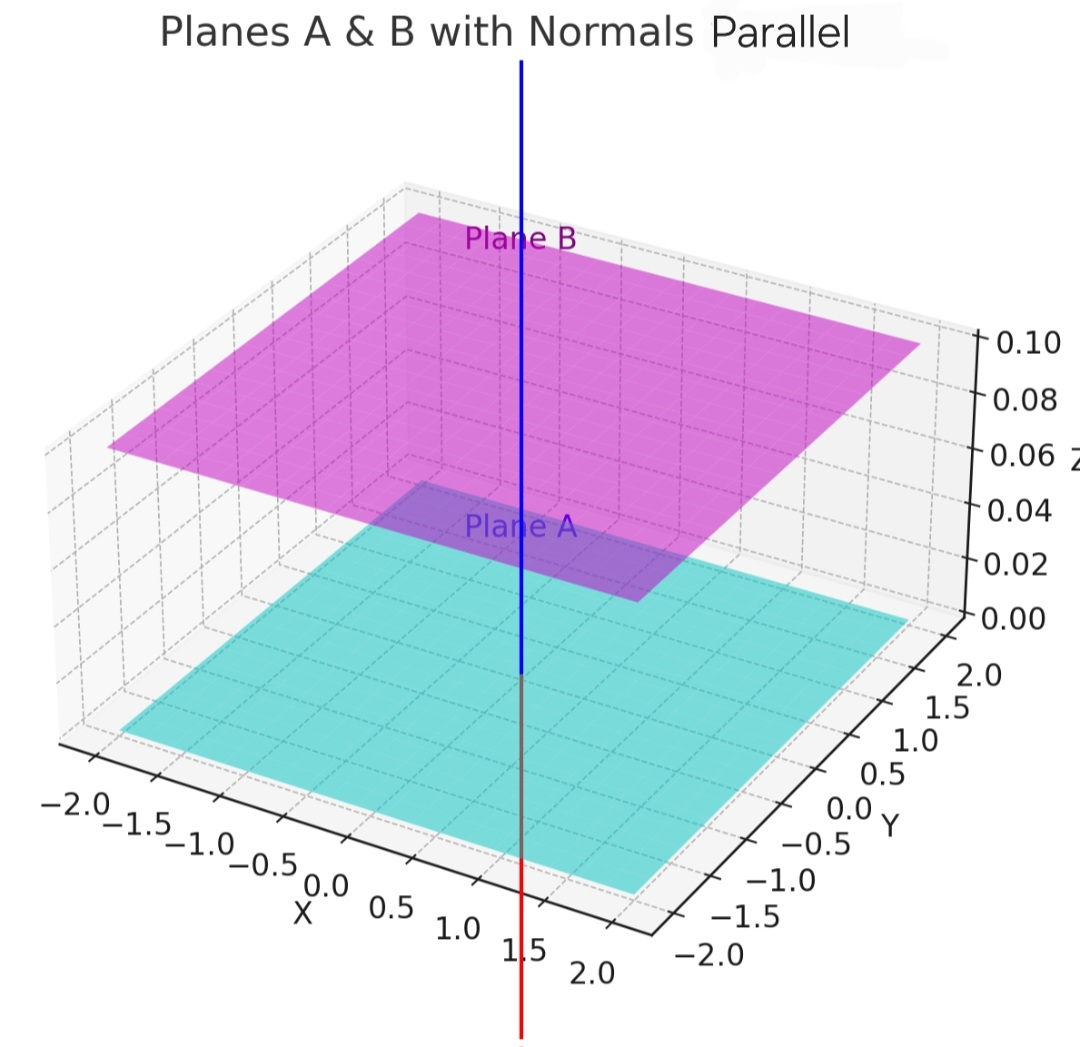
\includegraphics[width=0.75\columnwidth]{graph .jpg}
    \caption{Planes A and B}
    \label{fig:placeholder}
\end{figure}
\end{frame}

\end{document}